% ---- ETD Document Class and Useful Packages ---- %
\documentclass{ucetd}
\usepackage{subfigure,epsfig,amsfonts}
\usepackage{natbib}
\usepackage{amsmath}
\usepackage{amssymb}
\usepackage{amsthm}

%% abbreviations %%
\usepackage{enumitem}
\newlist{abbrv}{itemize}{1}
\setlist[abbrv,1]{label=,labelwidth=1in,align=parleft,itemsep=0.1\baselineskip,leftmargin=!}

%% figure floating %%
\usepackage{float}

%% caption formatting %%
\usepackage{caption}
\captionsetup[figure]{font=normal}

%% appendix package? %%
\usepackage{appendix}
\usepackage{chngcntr}
\usepackage{etoolbox}

\AtBeginEnvironment{subappendices}{%
\chapter*{Appendix}
\addcontentsline{toc}{chapter}{Appendices}
\counterwithin{figure}{section}
\counterwithin{table}{section}
}

%% shortcut commands %%
\usepackage{xspace}
\newcommand{\UP}{\textsuperscript{+}\xspace} % +
\newcommand{\UM}{\textsuperscript{--}\xspace} % -
\newcommand{\U}[1]{\textsuperscript{#1}\xspace} % superscript general
\newcommand{\aLP}{$\alpha$LP\xspace} % aLP
\newcommand{\aLPs}{$\alpha$LPs\xspace} % aLPs
\newcommand{\ab}{$\alpha_4 \beta_7$} % a4b7
\newcommand{\Rora}{Ror$\alpha$} % Rora
\newcommand{\RORa}{ROR$\alpha$} % RORa
\newcommand{\RORgt}{ROR$\gamma$t} % RORgt
\newcommand{\abT}{$\alpha\beta$T\xspace} % abT
\newcommand{\gdT}{$\gamma\delta$T\xspace} % gdT
\newcommand{\IFNg}{IFN$\gamma$\xspace} % IFNg
\newcommand{\CDte}{CD3$\varepsilon$} % CD3e
\newcommand{\Ragrg}{Rag\U{--/--} Il2rg\U{--/--}\xspace} %Rag-/-Il2rg-/-

%% Use these commands to set biographic information for the title page:
\title{Computational and Experimental Studies of Potassium Channel Folding}
\author{Kevin C. Song}
\department{Biophysical Sciences}
\divisiona{The Physical Sciences}
\divisionb{The Biological Sciences}
\degree{Doctor of Philosophy}
\date{August, 2018}

%% Use these commands to set a dedication and epigraph text
\dedication{To my wife,\\
			Louesa Song\\
		    To my parents,\\
            Dr. Byungho Song and Jeungen Yu\\
            To my sister,\\
            Kelly Song\\
            To my parents-in-law,\\
            Bruce Akin and Dr. S. Renea Akin\\
            }
\epigraph{"It doesn't matter how beautiful your theory is, it doesn't matter how smart you are. If it doesn't agree with experiment, it's wrong" - Richard Feynman}

\begin{document}
%% Basic setup commands
% If you don't want a title page comment out the next line and uncomment the line after it:
\maketitle
%\omittitle

% These lines can be commented out to disable the copyright/dedication/epigraph pages
\makecopyright
\makededication
\makeepigraph


%% Make the various tables of contents
\tableofcontents
\listoffigures
\listoftables

\acknowledgments
First, I would like to thank my academic advisors Dr. Beno\^{i}t Roux and Dr. Tobin Sosnick for their guidance throughout my thesis project. The nature of my thesis project was highly explorative, and without their patience and excellent guidance, this project would not have been able to be completed and fluorish. I really appreciate them both for giving me the intellectual freedom to learn how to be creative and teach me how to be a good scientist.

I would also like to thank my thesis committee members Dr. Eduardo Perozo and Dr. Andrei Tokmakoff for their insightful suggestions and discussions regarding my project. Specifically, I would like to thank Eduardo for his help with my understanding of membrane protein biochemistry better and I would like to thank Andrei for helping me understand protein kinetics better.

I have been extremely blessed with helpful and talented lab members, and especially, Yiling Zhang, Jing Li, Younghoon Koh, Michael Baxa, Adam Zmyslowski, Josh Riback

The University of Chicago Biophysics program has been invaluable to me, providing financial support as well as many friendships that will last throughout life. Michele Wittels, Julie Feder and Adam Hammond have provided me with assistance and constant support to ease. Eugene Leypunskiy, Herman Gudjonson, Vaughn Spurrier, and Boleslaw Osinski provided me with invaluable support and friendships throughout my tenure at the University of Chicago. I would not have been able to finish the work without their support

Last but not least, I would like to thank my family members Louesa Song, Dr. Byung Ho Song, Jeungen Yu, Bruce Akin, Dr. Renea Akin and Kelly Song for their constant support throughout life and 

\abstract
\par
This thesis connects the dynamics of Kv1.2 and KcsA potassium channel pore domain monomers to the kinetics of tetramerization. In simulations, monomers adopt multiple conformations with the three helices folded. NMR studies also find the monomers to be dynamic and structurally heterogeneous. However, a KcsA construct with a disulfide bridge engineered between the two transmembrane helices has an NMR spectrum with well-dispersed peaks, suggesting that the monomer can be locked into a native-like conformation. During tetramerization, FRET results indicate that monomers rapidly oligomerize upon insertion into liposomes, likely forming a dense protein-rich phase. Folding within this protein-rich phase occurs along separate fast and slow routes, with f ~ 40 and 1500 seconds, respectively. In contrast, constructs bearing the disulfide bond mainly fold via the faster pathway, suggesting that maintaining the TM helices in their native orientation reduces misfolding. Interestingly, folding is concentration independent in spite of the tetrameric nature of the channel, indicating that the rate-limiting step is unimolecular and occurs after monomer association in protein-rich phase. Finally, despite its name, the addition of KcsA’s C-terminal “tetramerization” domain does not improve the kinetics of tetramerization.

\mainmatter
% Main body of text follows 

%% INTRODUCTION %%


%% BEGIN INTRODUCTION %%

\chapter{Introduction}
\section{Membrane Protein Folding}
Membrane proteins are the cell's gateway to its environment. Using a variety of membrane proteins, a cell transmits information, receives nutrients, shapes itself and responds to outside signals. Membrane proteins reside in lipid membranes, and they constitute more than 30\% of the entire proteome. Despite its functional importance and its abundance, our understanding of biochemical and biophysical properties of membrane proteins are still immature because of the difficulties working with membrane proteins experimentally. Membrane proteins easily aggregate because of its high hydrophobicity, and without the correct membrane mimetics, the protein structures can be easily disturbed.

Generally speaking, membrane proteins can be sub-divided into 2 classes (\textbf{Fig. \ref{fig:intro_f1}}): $\alpha$-helical and $\beta$-barrel membrane proteins. $\alpha$-helical membrane proteins are mainly found in the plasma membrane of eukaryotes, the inner membranes of bacterial cells, and sometimes in the outer membranes of bacteria. They constitute between 20 - 25\% of all open reading frames. On the other hand, $\beta$-barrel membrane proteins are mostly found in the outer membranes of bacteria, mitochondria and chloroplasts, and they constitute only a few percent of all open reading frames. The folding processes for $\alpha$-helical and $\beta$-barrel membrane proteins are very different comprising different sets of chaperones and mechanisms.

\begin{figure}[!ht]
\begin{center}
	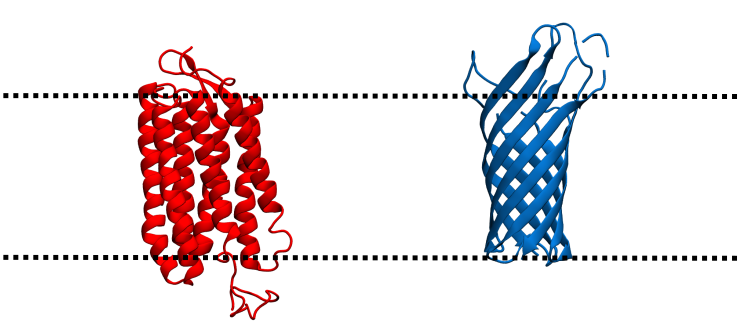
\includegraphics[width=\textwidth]{figures/introduction/Fig1/fig1.pdf}
\end{center}
	\caption{$\alpha$-helical versus $\beta$-barrel membrane protein}
Two representative structures of $\alpha$-helical and $\beta$-barrel membrane proteins are shown. Structure of bacteriorhodopsin (PDB ID: 1X0S) monomer is on the left in red, and OmpA (PDB ID: 1BXW) is shown on the right in blue. Hypothetical membrane boundaries are drawn in dashed black lines
	\label{fig:intro_f1}
\end{figure}

Individual $\alpha$-helices can be stable in the membrane as long as sidechains are hydrophobic enough; however, $\beta$-strands are not stable in the membrane because of exposed unsatisfied hydrogen donors and acceptors from the peptide backbone. Due to this difference in secondary structure, $\beta$-barrel membrane proteins insert and fold concurrently whereas $\alpha$-helical membrane proteins will insert one helix at a time and the helices rearrange to fold within the bilayer. In addition, $\beta$-barrel membrane proteins have been shown to fold reversibly from solution containing traditional denaturants such as urea and guanadine hydrochloride (GdnHCl) into lipids. (Fleming, Radford, Tamm, Rockwell) Because $\beta$-barrel membrane proteins can be monomeric and soluble in traditional denaturants, several proteins' (e.g. OmpA, OmpLA, OmpW, PagP) folding thermodynamics have been measured. In which, they found that they fold cooperatively by forming $\beta$ sheets at the lipid-water interface and insert. On the other hand, $\alpha$-helical membrane proteins are highly resistant to urea and GdnHCl, largely due to its hydrophobicity, and the denaturant of choice is sodium dodecyl sulfate (SDS) for folding studies of $\alpha$-helical membrane protein. With SDS, unfolded state of $\alpha$-helical membrane proteins still retain majority of its helicity. Because of this chemical property, most $\alpha$-helical membrane protein folding studies have focused on measuring folding thermodynamics and kinetics from SDS-unfolded states. 

The difference in folding mechanism is also reflected in how chaperones help these two classes of proteins fold. For $\beta$-barrel membrane proteins, BAM complexes have been shown to help them insert and fold by thinning the lipid bilayer thickness hence lowering the energy barrier to insert and fold. On the other hand, for $\alpha$-helical membrane proteins, ribosomes dock onto the SEC translocons and single helices are synthesized and inserted into the membrane one at a time as shown in \textbf{Figure \ref{fig:intro_f2}}. Many advances have been made in the field of $\beta$-barrel membrane proteins and there are excellent reviews available. (Fleming, Rockwell, Radford) Here in this thesis, the focus will be on the folding of $\alpha$-helical membrane proteins.

\begin{figure}[!ht]
\begin{center}
	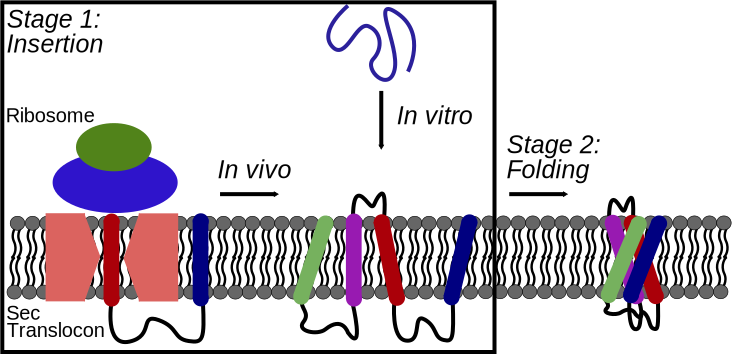
\includegraphics[width=\textwidth]{figures/introduction/Fig2/two_stage.pdf}
\end{center}
	\caption{Two-stage folding process for membrane protein folding.}
The first stage of the membrane protein folding process is insertion, where single helices are synthesized and inserted into the bilayer one at a time. As noted above, the insertion process is different for \textit{in vivo} and \textit{in vitro}. However, upon insertion of helices into the membrane, folding within the membrane is thought to process via the same pathway. 
	\label{fig:intro_f2}
\end{figure}

$\alpha$-helical membrane protein folding process is generally divided into 2 distinct stages (\textbf{Fig. \ref{fig:intro_f2}}). The first stage of membrane protein folding is called insertion, where the protein gets inserted into the membrane with native-like secondary structures. The exact mechanism on how a single helix transfers from inside the SEC translocon into the bilayer is not well understood yet, but the transfer is thought to happen via a lateral gate that opens in the translocon. Regardless, the insertion process is largely determined by the hydrophobicity of the peptide segment. Using amino acid hydrophobicity scales and sliding window averages, transmembrane segments can be well predicted. Yet, the prediction of final overall topology is still a difficult task. For some systems like LacY, the overall topologies can be flipped by changing the lipid compositions \textit{in vivo} and \textit{in vitro}.

After successful insertion of helices into the membrane, the helices begin to undergo a rearrangement process, which is described as folding within the membrane. This process is determined by many different forces including protein-protein and protein-lipid interactions. The major driving force for helix-helix interactions are not clear. Polar sidechain burial was thought of as a driving force for helix-helix associations; however, it was found



\section{Potassium Channels}
Potassium channels are found in all kingdoms of life. From bacteria to humans, potassium channels regulate the flow of K+ ions across cell membranes. In prokaryotes, these channels are responsible for cell growth and survival. In addition, biofilm, which is a community of bacterial cells, the microorganisms use potassium channels to communicate with each other. In higher order organisms like humans, potassium channels are used to drive muscle contraction and neuronal signaling.

The first structure of potassium channel was solved in 1998 by Roderick MacKinnon's lab, which he was awarded the Nobel Prize in Chemistry for in 2003. The structure showed that the pore is formed by juxtaposition of 4 subunits along the symmetry axis. The pore is lined with oxygen atoms from the backbone of the selectivity filter residues. Thes oxygen atoms provide binding sites for K+ ions as they pass through the pore. 


\section{Potassium Channel Folding}

%%\newpage
%%The aims of my studies are:
%%\begin{itemize}
%%\item Determine the structural state of potassium channel monomers in lipid bilayers
%%\item Determine the folding pathway of potassium channels
%%\end{itemize}

%% END INTRODUCTION %%


%%% BEGIN CHAPTER 2 MD Simulations and MSM %%%

%% Paper title page %%
\chapter{Molecular dynamics simulations and Markov state modeling of potassium channel monomers}

\section{Introduction}
In a previous 650 ns simulation, the wild-type (WT) Kv1.2 pore domain monomer in POPC lipid bilayer was stable in a native-like state with a C$\alpha$-RMSD below 3\AA. \cite{gajewski2011} However, this simulation was relatively short compared with the timescale of membrane protein dynamics, which could extend from the micro to the millisecond timescale. \cite{booth1995} To further explore the conformational flexibility of the monomer, we carried out 16.2 $\mu$s of simulations at T=353 K using the specialized Anton computer designed for MD. \cite{shaw2009} The relatively high temperature was chosen to accelerate sampling while still reproducing the thermodynamics of membrane protein folding. \cite{ulmschneider2014}

\section{Methods}

\subsection{Preparation of Kv1.2 and KcsA monomer simulations}
For all systems, the initial structures for the monomers were taken from the tetrameric Kv1.2 X-ray crystal structure (PDB ID: 2A79) using only the pore domain of 99 amino acids corresponding to residues 323 –- 421 in 2A79 structure. \cite{long2005} The starting structure for KcsA monomer simulations was taken from the tetrameric KcsA X-ray crystal structure (PDB ID: 1R3J). \cite{zhou2003} All systems were prepared by using CHARMM-GUI’s Membrane Builder module (www.charmm-gui.org). \cite{jo2007, jo2008, jo2009, lee2016, wu2014} For Kv1.2, each system contained 70 palmitoyl-oleoyl-phosphatidylcholine (POPC) molecules per leaflet totaling up to 140 POPC molecules in total, and for KcsA, each system contained 70 1,2-dimyristoyl-sn-glycero-3-phosphatidylcholine (DMPC) molecules per leaflet totaling up to 140 DMPC molecules to match the NMR sample conditions. All systems were hydrated by creating a water box 17.5 \AA above and below the protein’s maximum and minimum Z-positions. In addition, the system was neutralized with 150 mM KCl. The system comprised a total of approximately 45,000 atoms.

For Kv1.2 simulations, a number of different simulations are aggregated and summarized in the table below.
\begin{table}[h]
\centering
	\caption{Simulation summary for Kv1.2}
	\begin{tabular}{cccc}
	\hline
    Simulation & Temperature (K) & Number of Trajectories & Trajectory length \\
	\hline                                                                 
	\begin{tabular}[c]{@{}c@{}} Anton\\ simulation \end{tabular} & 353.15  & 1 & 16.2 $\mu$s\\
	GPU & 303.15  & 10 & $\sim$9.7 $\mu$s\\
	\begin{tabular}[c]{@{}c@{}} Adaptive\\ sampling \end{tabular} & 303.15  & 4685 & 0.06$\mu$s\\
	\hline
	\textbf{Total:} & \textbf{N/A} & \textbf{4803} & \textbf{394 $\mu$s}
	\end{tabular}
	\label{table:ch2_t1}
	\end{table}
	
For KcsA simulations, 5 independent simulations of KcsA WT monomer were carried out at T = 353 K to enhance sampling. All simulations were run with the parameters described in \textit{Amber16 simulations} section below, and each simulation was run up to 6 $\mu$s. In total 30 $\mu$s of KcsA WT simulations were accumulated.

\subsection{Anton simulations}
A long-time simulation run on Anton \cite{shaw2009} was prepared through energy minimization and equilibrating the initial simulation system using CHARMM36 force field with NAMD. \cite{phillips2005} Each system was energy minimized for 1,000 steps and was slowly equilibrated by reducing restraints on protein backbone, sidechain, and lipids gradually over 5 ns as recommended by CHARMM-GUI. After initial equilibrations with the restraints, the system was freed from all restraints and run for 100 ns before preparing the system for running simulations on Anton. The temperature was set to 353 K to increase sampling, which has been shown to capture thermodynamics more computationally efficiently. \cite{ulmschneider2014} All bonds involving hydrogen atoms were constrained by M-SHAKE. Cut-off values for van der Waals and short-range electrostatic interactions were optimized by Anton guesser script. For long-range electrostatic interaction calculations, k-space Gaussian split Ewald method with a 64 x 64 x 64 mesh was used, and the long-range electrostatics were calculated every 6 fs. The integration time step was 2 fs for all simulations, and the r-RESPA integration method was employed. \cite{tuckerman1992}

\subsection{Amber16 simulations}
For all systems that were simulated with Amber16 GPU, hydrogen mass repartitioning (HMR) scheme was applied, where all hydrogen masses were increased to 3, allowing simulation timestep to increase from 2 to 4 fs. The systems were prepared as described in System Preparation section using CHARMM-GUI, and \textit{parmed.py} program was used to modify the system to accommodate the HMR scheme. For temperature control, Langevin thermostat was used with friction coefficient of 0.3 and T=303 K, and coordinates were printed out every 50 ps. van der Waals force switching function was used with switch on at 10 Å and cutoff at 12 Å. Berensden barostat is used with semi-isotropic at pressure 1 atm. The Berensden coupling constant is set to 0.5 ps.

\subsection{Time-lagged independent component and Markov state model analysis}
For all molecular dynamics (MD) simulation analysis, MDTraj 1.9.0 and MSMbuilder 3.8.0 were used. \citep{harrigan2017, mcgibbon2015} In the first steps of constructing a Markov State Model (MSM), proper set of reaction coordinates, and discretized states within the chosen reaction coordinates are necessary. For these purposes, time-lagged independent component analysis (tICA) was used. For TICA, a set of relevant features must be inputted to generate a set of low-dimensional linear combination of the input features. For this featurization step, pairwise distances of all C-$\alpha$ atoms of all residues was used, which resulted in 4,831 features. Then through TICA, dimensionality reduction was performed. Based on implied timescale analysis, 3 TICs with the slowest relaxation timescale was found to adequately describe our system (\textbf{Fig. \ref{fig:ch2_f1}}). All simulations were transformed and projected onto the 3 TICs found.

\begin{figure}[!ht]
\begin{center}
	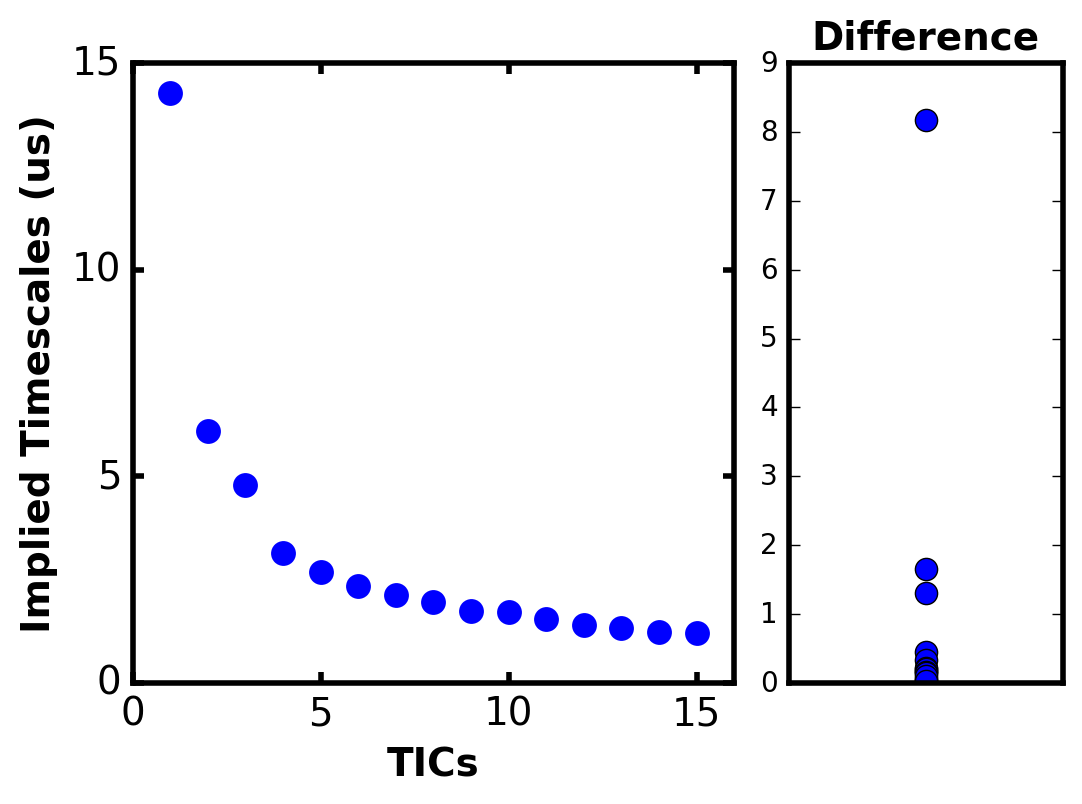
\includegraphics[width=\textwidth]{figures/chapter2/Fig2-1_implied_timescale.png}
\end{center}
	\caption{\textbf{TICA analysis of Kv1.2 simulations.} The implied relaxation timescale of each TIC is plotted versus the number of TICs. The first 3 TICs are chosen as reaction coordinates to represent the folding coordinates of the simulations.}
	\label{fig:ch2_f1}
\end{figure}

To discretize a set of relevant conformations within the TIC space, K-Center clustering algorithm was used. The cutoff value for number of states was determined using the elbow method, where the momentum (sum of squared distances of samples to their closest centers) was plotted against the number of states. The number of states where the decrease in inertia became marginally less than a certain threshold was found. For Kv1.2, k=150 states was found to be appropriate for clustering (\textbf{Fig. \ref{fig:ch2_f2}}).

\begin{figure}[!ht]
\begin{center}
	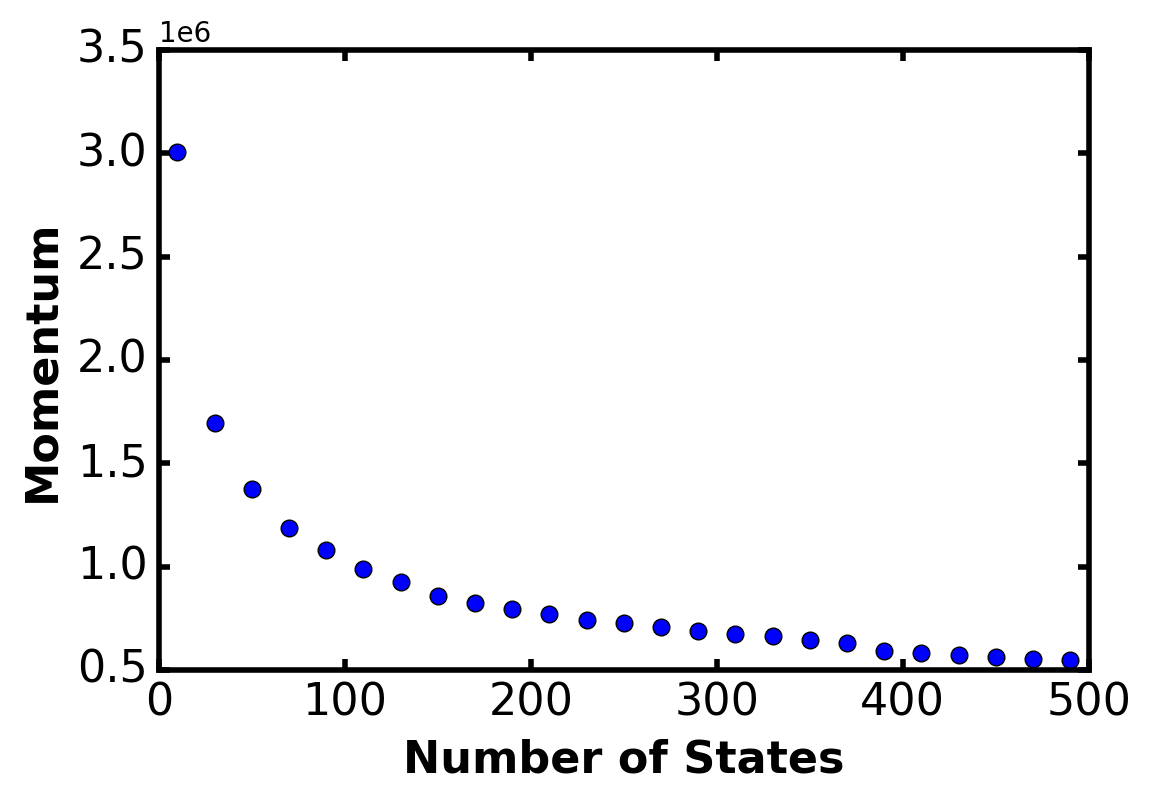
\includegraphics[width=\textwidth]{figures/chapter2/Fig2-2_momentum.png}
\end{center}
	\caption{\textbf{Change in momentum over number of states.} Momentum is calculated as the sum of distances between each data point and its nearest centroid. To determine the optimal number of states for K-Center clustering method, the number of states where the momentum value begins to plateau is chosen. For our studies, k=150 states deemed to be optimal.}
	\label{fig:ch2_f2}
\end{figure}

In order to construct a MSM, the optimal lag time was needed for constructing the count matrix. By the definition of Markovianity, as the lag time increases, the implied timescale of the Markov State Model should become invariant. Through our implied timescale analysis, lag time of 20 ns was found to be appropriate, and the Markov State Model was constructed using this value.
	
\subsection{Adaptive sampling scheme}
For adaptive sampling, initial MSM was constructed using the Anton trajectory. Adaptive sampling scheme described previously by Bowman et. al was used. \citep{bowman2010} Briefly, in each round of simulations, 50 states with the lowest MSM populations were chosen and those chosen centroid conformations were used as seeds for an additional 60 ns of AMBER16 simulations using the CHARMM36 force field with Hydrogen Mass Repartitioning (HMR) scheme. After each round of simulations, new sets of TICs were calculated and a new MSM was constructed. In total, we accumulated 394 $\mu$s of simulations which are then used to create the final MSM for WT Kv1.2 monomer. 

\section{Results and Discussion}
\subsection{Potassium channel monomers are dynamical}
In a previous 650 ns MD simulation, the wild-type (WT) Kv1.2 pore domain monomer in POPC lipid bilayer was stable in a native-like state with a C$\alpha$-RMSD below 3 \AA. \cite{gajewski2011} However, this simulation is relatively short compared with the micro to the millisecond timescale of membrane protein dynamics. \citep{booth1995} To further explore the monomer’s conformational flexibility, we carried out 16.2 $\mu$s of simulations at T=353 K using the specialized Anton computer designed for simulations.\citep{shaw2009} The relatively high temperature was chosen to accelerate sampling while still reproducing the thermodynamics of membrane protein folding.

\begin{figure}[!ht]
\begin{center}
	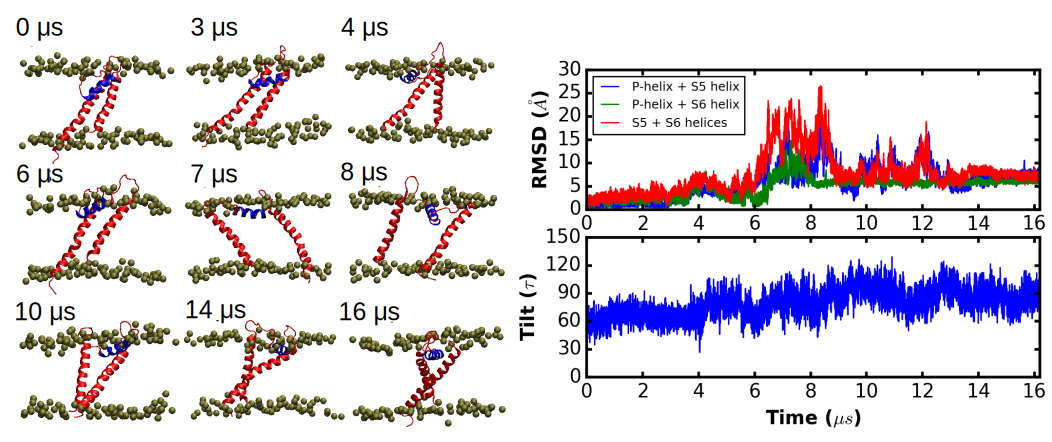
\includegraphics[width=\textwidth]{figures/chapter2/Fig2-3_anton.pdf}
\end{center}
	\caption{\textbf{Molecular dynamics simulation of Kv1.2 pore domain monomer in POPC lipid bilayer ran for 16.2 $\mu$s on Anton.} \textbf{Left}: Selected snapshots. \textbf{Right}: Pair-wise C$\alpha$-RMSD values for pairs of helices and the tilting angle of the pore helix.}
	\label{fig:ch2_f3}
\end{figure}

During the first 3 $\mu$s of the simulation, the structure was stable with a C$\alpha$-RMSD to the initial (native-like) state below 4 \AA (\textbf{Fig. \ref{fig:ch2_f3}}). Nevertheless, the p-helix became more parallel to the membrane during the first microsecond with the tilt angle increasing from 47$^{\circ}$ to 80$^{\circ}$ relative to the surface normal (\textbf{Fig. \ref{fig:ch2_f3}}). The average tilt angle over the entire 16.2 $\mu$s was 80$^{\circ}$ $\pm$ 10$^{\circ}$. At 4 $\mu$s, the 2 TM helices started to separate laterally with slightly different tilt angles due to their different lengths, leading to overall C$\alpha$-RMSD values greater than 4 \AA. 

Between 6 and 8 $\mu$s, all three helices separated (Fig. S1), but the p-helix remained helical and stayed nearly parallel to the membrane surface. This orientation allowed the polar and charged residues in the pore loop region to become more solvent exposed, while segregating the nonpolar residues. This result is qualitatively consistent with the previous thiol-labeling results, which indicated that the p-helix remains helical and resides at the water-lipid interface. \citep{delaney2014} Based on short simulations (650 ns) and thiol-labeling experimental data, the Kv1.3 monomer was inferred to retain native-like tertiary contacts. \citep{gajewski2011} In the long Anton simulation, however, the monomer is stable up to 3 $\mu$s with RMSD less than 4 \AA but also explores many other non-native states.

After 8 $\mu$s of simulations, residue D381 formed a salt bridge with a K398 that resides on top of the carboxy-terminal S6 helix. This salt bridge persisted for the last 8 $\mu$s and stabilized the interactions between the S6 and the p-helix. The amino terminal S5 helix eventually drifted towards the complex formed by the S6 with the p-helix, to produce an alternate structure. Interestingly, the salt bridge formed between the p-helix and S6 mimics a salt-bridge that is formed between p-helix of one monomer with the S6 helix of an adjacent monomer in the native tetramer (which does exist in the simulations). Salt bridges are known to be overly stabilized in simulations25 so the longevity of the D381-K398 bridge may be unrealistic. Nevertheless, the monomer spent a majority of time with the three helices in a non-native arrangement.

\subsection{Markov state modeling of Kv1.2 and KcsA monomer simulations}
To obtain a better estimate of the conformation ensemble of Kv1.2 monomers, an analysis based on Markov state models (MSM) was performed using 3 sets of simulations (\textbf{Table. \ref{table:ch2_t1}}): (1) 16.2 $\mu$s Anton simulation at T=353 K; (2) 10 independent 9 $\mu$s long simulations starting from the native state at T=303 K; (3) 100 rounds of adaptive sampling simulations (SI Methods) at T=303 K. A total of 394 $\mu$s of simulations was accumulated and used for time-structure Independent Component Analysis (TICA) and MSM analysis. \citep{molgedey1994, noe2015, noe2016, perezHernandez2013, schwantes2013}

Based on the MSM analysis, the population of native-like structures (C$\alpha$-RMSD < 4 Å) converged at 18\% (Fig. 2B, S2 bottom). This result further supports the finding that the native-like monomer conformation is present but is not predominant in lipid bilayer. While the two TM helices and the p-helix retained their helicity in all structures, the monomer prefers to be partially disordered. The p-helix remained parallel to the water-lipid interface, which is consistent with the thiol-labeling results. \citep{gajewski2011} Overall, the monomer existed as a heterogeneous ensemble of contacting and non-contacting helices.

To compare with the Kv1.2 simulations, and to enable a direct comparison with our experiments, simulations were conducted on KcsA pore domain monomers without the C-terminal tetramerization domain (PDB ID: 1R3J, residues 22 -- 124). The pore domain of KcsA and Kv1.2, comprising the pore loop and the 2 TMs, have 31\% sequence identity. This suggests that the gross dynamical features of the two proteins should be qualitatively similar. Five 5 $\mu$s trajectories were initiated from the native state at T=353 K. To compare with the Kv1.2 simulations, the KcsA trajectories were first projected onto the same set of TICs obtained from the Kv1.2 simulations and also aggregated with the Kv1.2 simulations to create a new set of common microstates. Although the sampling was less extensive as compared to Kv1.2, the general behavior of KcsA was similar. The KcsA monomer adopted a variety of native-like (44\%) and non-native structures, albeit with the three helices separated less than Kv1.2 helices (Figs. S5, S6). 

\section{Conclusion}

%% REVERT FIGURE NUMBERING %%
\renewcommand\thefigure{\thechapter.\arabic{figure}} 

%%% END CHAPTER 2 MD MSM %%%


%%% BEGIN CHAPTER 3 Design of fast folding potassium channel mutant %%%

%% Paper title page %%
\chapter{Biochemical preparation of KcsA monomers and Design of fast folding KcsA mutant}
\section{Introduction}
Bacterial potassium channel, KcsA, is an extremely stable tetramer. \citep{valiyaveetil2002semi, barrera2005, barrera2008, heginbotham1997, valiyaveetil2002lipids}	Conventional denaturing reagents such as urea and guanadine do not unfold KcsA. \citep{valiyaveetil2002lipids} Sodium dodecyl sulfate (SDS) detergent is a harsh denaturing reagent for most soluble and membrane proteins; however, even SDS alone does not unfold KcsA. Only with SDS and boiling of the protein sample at 90 $^{\circ}$C for more than 10 minutes can disrupt the KcsA tetramer. So, the question is, how do we get stable monomers for biophysical studies?

In the first part of Chapter 3, a protocol for preparing KcsA monomer is presented, which are adopted from \citep{shenkarev2013} and \citep{devaraneni2011}. WT KcsA monomers were inserted into lipid nanodiscs as well as lipid bicelles for NMR studies. Through NMR and simulations, we find that the WT KcsA monomer is highly dynamic and exists in a structurally diverse ensemble of states. To stabilize the native-like state in monomers, we engineer a disulfide bond at the end of the two TM helices. This disulfide-bonded (CC) KcsA mutant monomer displays a much more native-like structure.

\section{Methods}
\subsection{KcsA expression and purification}
\subsubsection{Expression}
For KcsA expression with no isotope labeling, the protocol was adopted from \citep{tilegenova2016}. XL10-GOLD \textit{E. coli} competent cells were transformed with pQE70 KcsA WT with C-terminal 6xHis-tag using the heat shock method and grown overnight at 37 $^{\circ}$C with 1\% glucose and ampicillin (200 $\mu$g/mL). This overnight culture was used to inoculate LB media supplemented with 0.5\% glycerol, 0.2\% glucose and ampicillin (200 $\mu$g/mL) at a final concentration of 1\% v/v. Once this culture reached OD$_{600}$ $\sim$ 0.6 and they were cooled down to 29 $^{\circ}$C for 1 hour. Then, protein expression was induced with 0.1 mM Isopropyl $\beta$-D-1-thiogalactopyranoside (IPTG), 10mM BaCl2 (K+ channel blocker) and 0.2 $\mu$g/mL ampicillin. Cells were incubated overnight at 29 $^{\circ}$C and harvested after 14 -- 18 hours of growth by centrifuging at 9,000 RCF for 15 minutes at 4 $^{\circ}$C. The pellet was stored in -70 $^{\circ}$C until purification.

For expressions with isotope labeling for NMR studies, the protocol was adopted from \citep{bhate2013}. JM83 \textit{E. coli} competent cells were transformed with pASK90 KcsA with N-terminal 6xHis-tag and grown overnight at 37 $^{\circ}$C with ampicillin (200 $\mu$g/mL). The overnight culture was used to inoculate a 100 mL of LB media with ampicillin (200 $\mu$g/mL) and was grown until OD$_{600}$ reached 0.5. This culture was then used to inoculate 4 L of LB media by adding 1\% of the total volume. The 4 L of LB were grown until OD$_{600}$ reached $\sim$ 0.9 and were spun down at 4,000 RCF for 10 minutes at 4 $^{\circ}$C. The biomass was quadrupled by combining cell pellets from 4 L of LB media into 1 L of M9 media. The pellet was resuspended with 40 mL of M9 media and returned to 1 L of M9 media. The cells were allowed to acclimate for an hour at 37 $^{\circ}$C and then were induced with 0.2mg/L anhydrotetracycline (aTC). Pellets were harvested 12 –- 14 hours later by spinning down at 9,000 RCF for 15 minutes at 4 $^{\circ}$C. After the pellet was spun down, the pellet was frozen in -70 $^{\circ}$C until purification. 

For the M9 media, the ingredients are shown in Tables \ref{table:ch3_t1}, \ref{table:ch3_t2} and \ref{table:ch3_t3}. For vitamin stock solution, one multi-purpose vitamin purchased from CVS is crushed using mortar and pestle. The crushed vitamin is then solubilized in deionized water in 20 mL volume. This solution is then sterile filtered and stored in -20 $^{\circ}$C. When making the M9 media, Na$_{2}$HPO$_{4}$, KH$_{2}$PO$_{4}$, NaCl are first mixed together and autoclaved. Rest of the ingredients are added after autoclave.
\begin{table}[h]
\centering
	\caption{Ingredients for 1L of M9 media}
	\begin{tabular}{cc}
	\hline
	Ingredients & Amount \\
	\hline
	Na$_{2}$HPO$_{4}$     & 12.8 g  \\
	KH$_{2}$PO${4}$      & 3 g \\
	NaCl & 0.5 g \\
	Solution C & 20 mL \\
	MgSO$_{4}$ & 0.1 g \\
	CaCl$_{2}$ & 0.01 g \\
	FeCl$_{2}$ & 0.01 g \\
	Thiamine & 0.01 g \\
	Glucose & 3 g \\
	NH$_{4}$Cl & 1 g \\
	L-Proline & 1 g \\
	Vitamin Stock & 2 mL \\
	Ampicillin & 0.2 g \\
	\hline
	\end{tabular}
	\label{table:ch3_t1}
	\end{table}

\begin{table}[!htb]
%\centering
    \begin{minipage}{.5\linewidth}
	  \caption{1 L of Solution C \\ adjust pH to 6.7}
      \centering
		\begin{tabular}{cc}
		\hline
		Ingredients & Amount \\
		\hline
		KOH & 7.3 g  \\
		Metal 44 & 50 mL \\
		Nitrilotriacetic acid & 10 g \\
		MgCl$_{2}$ 6H$_{2}$O & 24 g \\
		CaCl$_{2}$ 2H$_{2}$O & 3.335 g \\
		\hline
		\end{tabular}
		\label{table:ch3_t2}
    \end{minipage}
    \begin{minipage}{.5\linewidth}
		\caption{100 mL of Metal 44 Solution, \\store in dark glass bottle at 4 $^{\circ}$C}
		\centering
		  \begin{tabular}{cc}
	  	  \hline
		  Ingredients & Amount \\
 	      \hline
	      K$_{2}$EDTA 2H$_{2}$O  & 0.327 g  \\
          ZnCl$_{2}$ & 0.522 g \\
		  FeCl$_{2}$ 4H$_{2}$O & 0.502 g \\
		  MnCl$_{2}$ 4H$_{2}$O & 0.18 g \\	
		  (NH$_{4}$)$_{6}$Mo$_{7}$O$_{24}$ 6H$_{2}$O & 0.0185 g \\
		  CuCl$_{2}$ 2H$_{2}$O & 0.0156 g \\
		  Co(NO$_{3}$)$_{2}$ 6H$_{2}$O & 0.0248 g \\
		  Boric Acid & 0.0114 g \\
		  \hline
		  \end{tabular}
		  \label{table:ch3_t3}
    \end{minipage} 
\end{table}

\subsubsection{Purification}
For purification, the frozen pellets were resuspended in buffer A (50 mM HEPES, 200 mM KCl, pH 7.0) with 1 mM phenylmethylsulfonyl fluoride (PMSF), 3 mg of DNAse A (Goldbio) per liter of culture, and 0.4 mM MgSO$_{4}$. The cells were lysed through 3x passage through french press, and the lysed cells were spun down at 158,000 RCF for 30 minutes at 4 $^{\circ}$C. The pellet was resuspended in buffer A with 10 mM n-dodecyl $\beta$-D-maltoside (DDM) and 1 mM PMSF. The mixture was rotated at room temperature for 1 hour to extract and solubilize KcsA in DDM. Then, the mixture was spun down at 185,000 RCF for 1 hour at 4 $^{\circ}$C. Supernatant was incubated with Talon Metal Affinity Co2+ resins and rotated at room temperature for 1 hour. The resins were then collected by gravity and the flow through was discarded. The columns were washed with 15 bed volumes of Buffer A + 1 mM DDM + 10 mM imidazole and the proteins were eluted with Buffer A + 1 mM DDM + 500 mM imidazole.

For full-length KcsA constructs, protein in elution solution was further purified by size-exclusion chromatography on Superdex 200 Increase column that was pre-equilibrated with Buffer containing 50 mM NaPi, 100 mM NaCl, 1 mM DDM, pH 7. For KcsA $\Delta$125 constructs, full length KcsA constructs were first trypsinized with $\alpha$-chymotrypsin (Sigma Aldrich) at 4 $^{\circ}$C overnight with 1:50 (chymotrypsin:KcsA) ratio. Then, the digested KcsA was further purified through size-exclusion chromatography (SEC) with Superdex 200 Increase column. 

\subsection{Design and production of fast folding KcsA mutant}
Based on previous simulations of WT Kv1.2 and KcsA monomers as well as NMR results shown in \textit{Results} section of this chapter, potassium channel pore domain monomers seemed to be highly dynamic and structurally heterogeneous. In order to limit the dynamical nature of WT KcsA monomer, we introduce a disulfide bridge at the end of the two TM helices to limit its dynamical nature. The residues chosen for mutations are A29 and A109, and both were mutated using the QuickChange protocol. For expression and purification, the protocol is identical to expression and purification of WT KcsA discussed in the previous section.

\subsection{KcsA monomer preparation}
\begin{figure}[!ht]
\begin{center}
	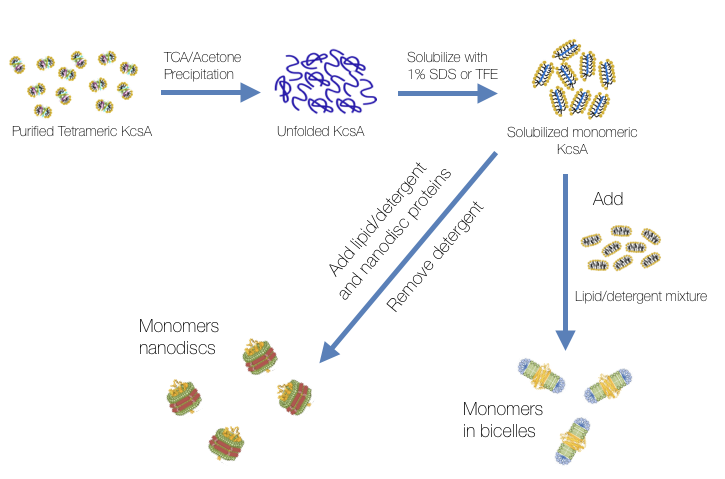
\includegraphics[width=\textwidth]{figures/chapter3/monomer_prep.png}
\end{center}
	\caption{\textbf{Protocol for preparing monomeric KcsA in nanodisc or bicelle}}
	\label{fig:ch3_f1}
\end{figure}

For preparing monomer samples, we follow the protocol highlighted in Figure \ref{fig:ch3_f1}. Purified tetrameric KcsA after SEC step are all pooled together, and they are precipitated by adding 15\% v/v tricholoroacetic acid (TCA) to the samples. The precipitated samples were frozen at -70 $^{\circ}$C for 30 minutes. Then, the frozen samples were spun down at 16,200 RCF for 30 minutes at 4 $^{\circ}$C. Supernatant was removed, and washed with chilled (-20 $^{\circ}$C) acetone. Precipitates were resuspended, vortexed for 30 seconds, and incubated at -20 $^{\circ}$C for 30 minutes until spin down at 16,200 RCF for 15 minutes at 4 $^{\circ}$C. This acetone wash step was repeated 3 times. The final precipitate was dried under air until all acetone evaporated, and the precipitate was stored in -80 $^{\circ}$C until usage. For solubilizing the precipitated monomers, either 1\% SDS or 100\% TFE is used.

\subsubsection{KcsA monomer in nanodisc}
The protocol for kinetically trapping KcsA monomer in nanodisc was adopted from \citep{hagn2013} and \citep{ritchie2009}. First, 0.5\% SDS-solubilized KcsA monomers is mixed with 1,2-dimyristoyl-sn-glycero-3-phosphoglycerol (DMPG) and sodium cholate. Typically, DMPG is mixed with cholate at ratio of 1:2. Optimal protein to lipid ratio was determined empirically at 1:5 by checking the monodispersity of size-exlusion chromatography (SEC) elution profile. After an hour of mixing at room temperature, 1 g of Biobead SM-2 is added per mL of nanodisc mixture. Then, the mixtures with Biobeads is further mixed for overnight at room temperature. Biobeads were removed by centrifugation and nanodiscs were further purified by SEC using Superdex 200 Increase column. 

\subsubsection{KcsA monomer in bicelle}
KcsA monomers in bicelles were prepared in q=0.3 DMPC:DHPC bicelles using following procedure. Bicelle mixture was first prepared by adding 1:3 molar ratio of DMPC or POPC to DHPC (both solubilized in chloroform) at final lipid concentration of 10\% w/v in the NMR sample. Chloroform was evaporated under stream of nitrogen and further removed under vacuum for 3 –- 4 hours. This procedure resulted in a thin lipid film, which was resolubilized in 2,2,2-trifluoroethanol (TFE). WT KcsA $\Delta$125 precipitate is solubilized in TFE and mixed into the lipid TFE mixture. TFE was evaporated under a stream of nitrogen until a thin film formed around the glass tube and was further evaporated by placing the tube under vacuum overnight. Then, the thin lipid film was rehydrated with buffer of choice and vortexed for 30 seconds. Typically for NMR, the buffer contained 20 mM NaPi, 50 mM NaCl, 0.03\% NaN$_{3}$, and pH6.5. 

\subsection{Nuclear magnetic resonance (NMR) measurements of KcsA}
NMR spectra were acquired on Bruker AVANCE IIIHD 600 MHz NMR spectrometer equipped with a room temperature TXI probe. [$^{1}$H, $^{15}$N]-TROSY HSQC experiments were run at T=323 K. To obtain rotational correlation times, $\tau_{c}$, [15N, 1H]-TRACT experiments were performed. \citep{lee2006, cavanagh2007, cho1999, nesg2011, pond2012} 

\subsection{KcsA CC simulations and MSM analysis}
The starting structure for KcsA monomer simulations was taken from the tetrameric KcsA X-ray crystal structure (PDB ID: 1R3J). Mutations were made at A29C and A109C for the disulfide mutant simulations, and disulfide bond was created using CHARMM-GUI’s PDBReader module. All systems were prepared by using CHARMM-GUI’s Membrane Builder module (www.charmm-gui.org)64-68. Each system contained 70 1,2-dimyristoyl-sn-glycero-3-phosphatidylcholine (DMPC) molecules per leaflet totaling up to 140 DMPC molecules to match the NMR sample conditions. All systems were hydrated by creating a water box 17.5 Å above and below the protein’s maximum and minimum Z-positions. In addition, the system was neutralized with 150 mM KCl. The system comprised a total of approximately 45,000 atoms. 5 independent simulations of KcsA WT monomer and 5 simulations of KcsA CC mutant monomer were carried out at T = 353 K to enhance sampling. All simulations were run with the parameters described in Methods section with AMBER16 GPU, and each simulation was run up to 6 $\mu$s. In total 30 $\mu$s of KcsA WT simulations and 30 $\mu$s of KcsA CC simulations were accumulated.

For MSM analysis, all KcsA simulations were first projected onto the TIC space created by Kv1.2 simulations. KcsA monomer has 103 residues in total whereas Kv1.2 pore domain has 99 residues. In order to project KcsA monomer simulations, C$\alpha$ atoms were aligned to Kv1.2 structure. The final corresponding residues in KcsA were from residues 24 to 122, which were used for TICA projection. After projecting KcsA simulations onto the same TIC space as Kv1.2, all simulations were combined in order to create the same number of microstates using K-Center clustering algorithm. After the same microstates were created, Markov state model constructions were done as described in SI Methods. However, MSM was constructed separately for Kv1.2, KcsA WT and KcsA CC using the same set of microstates.

\section{Results and Discussion}
\subsection{WT KcsA monomers are structurally diverse}

Expression and purification of KcsA tetramers is straightforward. Many labs can reliably produce large amounts of KcsA for biophysical studies. \citep{chill2007, valiyaveetil2002semi, barrera2005, tilegenova2016, bhate2013, takeuchi2007, cortes1997} KcsA $\Delta$125 constructs are prepared by incubating KcsA full-length (FL) constructs with $\alpha$-chymotrypsin at 1:50 ratio overnight at 4 $^{\circ}$C. Then, the KcsA $\Delta$125 are purified from chymotrypsin by size-exclusion chromatography (SEC) with Superdex 200 Increase column as shown in Figure \ref{fig:ch3_f2}B.

\begin{figure}[!ht]
\begin{center}
	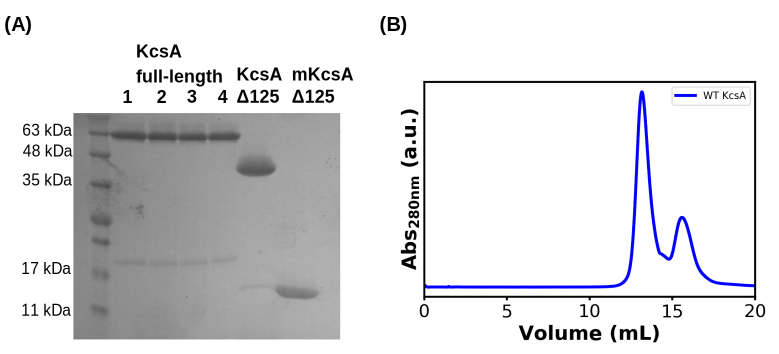
\includegraphics[width=\textwidth]{figures/chapter3/wtkcsa_gel_sec.pdf}
\end{center}
	\caption{\textbf{Purification of KcsA} \textbf{(A)} SDS-PAGE gel with KcsA full-length (FL), KcsA $\Delta$125, monomeric KcsA (mKcsA) $\Delta$125. \textbf{(B)} Elution profile of WT KcsA $\Delta$ tetramer with chymotrypsin. KcsA $\Delta$125 elutes around 13 mL and chymotrypsin elutes near 16 mL.}
	\label{fig:ch3_f2}
\end{figure}

KcsA monomers are prepared by trichloroacetic acid (TCA)/Acetone precipitation protocol as discussed in \textit{Methods} section. The precipitate monomers can be solubilized in 0.5\% SDS and is shown to run as 13 kDa on SDS-PAGE (\textbf{Fig. \ref{fig:ch3_f2}}). The monomers were then transferred to nanodisc or bicelle for NMR studies.

\begin{figure}[!ht]
\begin{center}
	\includegraphics[width=\textwidth]{figures/chapter3/wt_nmr.pdf}
\end{center}
	\caption{\textbf{[$^{15}$N-$^{1}$H]-TROSY-HSQC spectra of KcsA WT.}  \textbf{(A)} HSQC of KcsA $\Delta$125 solubilized in MSP1D1 $\Delta$H5 nanodisc is shown. \textbf{(B)} HSQC of KcsA $\Delta$125 solubilized in q=0.3 DMPC:DHPC bicelle is shown.}
	\label{fig:ch3_f3}
\end{figure}

NMR spectra of WT KcsA in either MSP1D1 $\Delta$H5 or q=0.3 DMPC:DHPC bicelle do not show well-resolved peaks in general. In fact, for WT KcsA solubilized in bicelle easily forms soluble aggregates in the NMR sample conditions. In Chapter 2, we found that Kv1.2 and KcsA monomers seem to be structurally diverse through MD simulations and Markov state model analysis. Given our NMR spectra and the computational modelling results, we suspect that the WT KcsA monomers are structurally heterogeneous in lipid bilayers. 

\subsection{Designing more native-like KcsA mutant}

With the KcsA mutant

\begin{figure}[!ht]
\begin{center}
	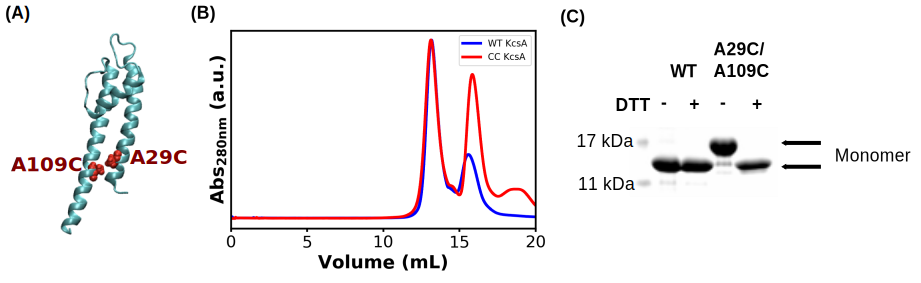
\includegraphics[width=\textwidth]{figures/chapter3/cc_sec_gel.pdf}
\end{center}
	\caption{\textbf{[$^{15}$N-$^{1}$H]-TROSY-HSQC spectra of KcsA WT.}  \textbf{(A)} HSQC of KcsA $\Delta$125 solubilized in MSP1D1 $\Delta$H5 nanodisc is shown. \textbf{(B)} HSQC of KcsA $\Delta$125 solubilized in q=0.3 DMPC:DHPC bicelle is shown.}
	\label{fig:ch3_f4}
\end{figure}

\subsection{NMR of potassium channel monomers}

\begin{figure}[!ht]
\begin{center}
	\includegraphics[width=\textwidth]{figures/chapter3/nmr.pdf}
\end{center}
	\caption{\textbf{Simulation comparison between Kv1.2 and KcsA.} \textbf{(A)} Number of contacts between the 2 transmembrane helices are plotted as a function of simulation time. \textbf{(B)} RMSD of the overall monomer is plotted as a function of time. \textbf{(C)} Kv1.2 and KcsA simulations are projected onto the same TIC space. Markov state model is made using the same set of microstates and the correponding free energy surface is plotted}
	\label{fig:ch3_f5}
\end{figure}

\section{Conclusion}

%% REVERT FIGURE NUMBERING %%
\renewcommand\thefigure{\thechapter.\arabic{figure}} 

%%% END CHAPTER 2 Design of fast folding potassium channel mutant %%%

%%% BEGIN CHAPTER 4 MICROARRAY %%%

%% Paper title page %%
\chapter{Folding and misfolding of potassium channel monomers during assembly and tetramerization}
\section{Introduction}

In Chapter 3, we developed a KcsA monomer mutant that retains its native-like structure more than the wild-type (WT) does by engineering a disulfide bridge near the ends of the 2 transmembrane (TM) helices. Here in this chapter, we compare the folding kinetics of WT and the disulfide-bridged (CC) KcsA mutant with and without the C-terminal "tetramerization" domain. The refolding studies reveal several interesting aspects about potassium channel folding. First, the WT KcsA folding displays a biphasic kientic behavior with fast and slow processes with $\tau_{f} \sim$ 50 and 1400 seconds, respectively. However, in the CC mutant, only the fast process is present, suggesting that locking the 2 TM helices with a disulfide bond minimizes its proclivity to misfold. Secondly, WT and CC without the C-terminal "tetramerization" domain does not have any concentration dependence despite the fact that the native state is a tetramer. Thirdly, WT and CC with the C-terminal "tetramerization" domain does fold with concentration dependence in the range of 1 - 10 $\mu$M concentration. Lastly, through ensemble FRET measurements, we propose that KcsA monomers form a dense protein-rich phase in the membrane first and fold into native structures from this phase.

\section{Methods}
\subsection{Refolding KcsA protocol}

Refolding experiments were adapted from Komarov et al.17 Briefly, desired amounts of soyPC lipids (Avanti) was dried under nitrogen gas to form a thin film and further dried under vacuum overnight. Dried lipid mixture was brought up to 10 mg/mL concentration by rehydrating the thin lipid film with Buffer B (50 mM NaPi, 100 mM NaCl, pH 6.5). This mixture was rotated for 30 minutes at room temperature, and then, in order to form small unilameller vesicles, the mixture was sonicated using a bath sonicator for 15 minutes at room temperature.

\begin{figure}[!ht]
\begin{center}
	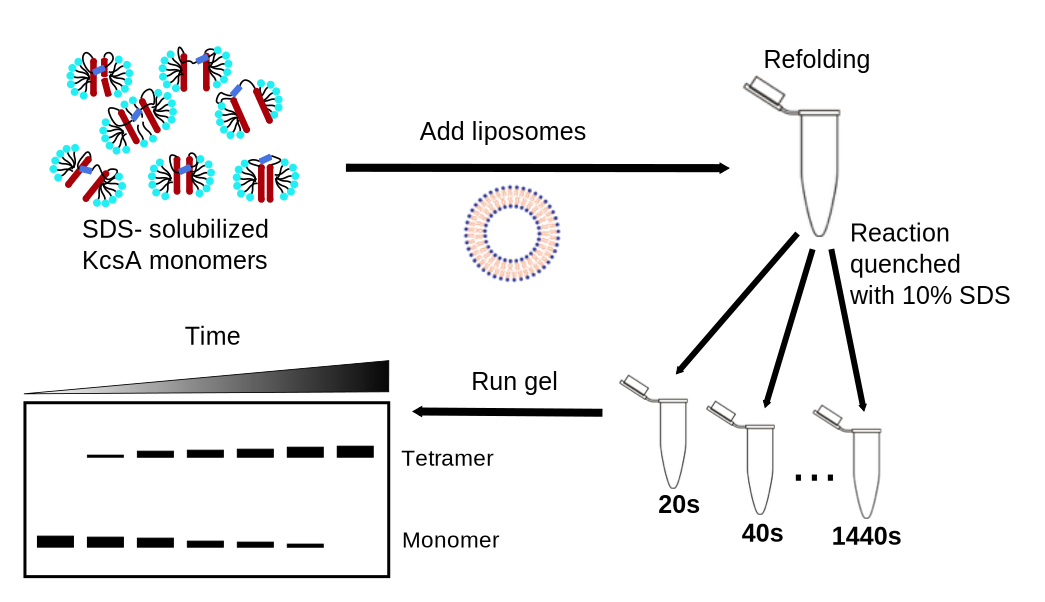
\includegraphics[width=\textwidth]{figures/chapter4/Fig4-1_refolding_protocol.pdf}
\end{center}
	\caption{\textbf{Structure of KcsA (PDB ID: 1R3J) shown from different angles}. \textbf{(A)} KcsA shown from the extracellular side of the membrane. \textbf{(B)} KcsA shown from the side. \textbf{(C)} KcsA viewed from the side with 2 monomers removed for better visualization of the selectivity filter. The oxygen atoms lining the selectivity region is rendered in Licoriche mode and the protein structures are rendered in New Cartoon mode in VMD. Each monomer of KcsA is colored in grey, blue, orange and red.}
	\label{fig:ch4_f1}
\end{figure}

Prior to refolding, precipitated KcsA $\Delta$125 monomers were solubilized in 0.5\% SDS in Buffer B with roughly protein concentrations of ~1.8 mg/mL. To initiate refolding, the protein mixture was diluted 10-fold into the refolding buffer containing asolectin vesicles. Then, at each time point a small aliquot of the refolding mixture was taken out and the reaction was quenched by diluting into 10\% SDS in Buffer B at 1:2 ratio. These quenched reaction mixtures were then run on a Novex Tris-glycine 4 – 20\% SDS-PAGE gel (ThermoFisher).

\subsection{Kinetics analysis}
	For analysis, gel images were taken with a Bio-rad ChemiDoc instrument. Then, the image was processed using ImageLab software to enhance the contrast between the protein bands and the background. For quantifying tetramer to monomer ratio, ImageJ software’s gel analysis tool was used. Each lane was normalized to itself by calculating the $\frac{[Tetramer]}{[Tetramer]+[Monomer]}$ ratio. For fitting, a double exponential function in the form of
	\begin{equation} a-be^{-\frac{t}{c}}-de^{-\frac{t}{e}} \end{equation}
was used and fitted using Scipy.optimize package in python.

\subsection{F\"{o}rster resonance energy transfer (FRET) of KcsA in liposomes}
For the site of dye conjugation, L86 in KcsA was chosen. The L86C mutation was obtained using the QuickChange protocol. Protein was expressed and purified as discussed above. Conjugation of either Cy3 or Cy5 maleimide (Kerafast) was done by overnight incubation at 4 $^{\circ}$C. Excess dye molecules were removed by size-exclusion chromatography using Superdex 200 Increase column (\textbf{Fig. \ref{fig:ch4_f2}} 

\begin{figure}[!ht]
\begin{center}
	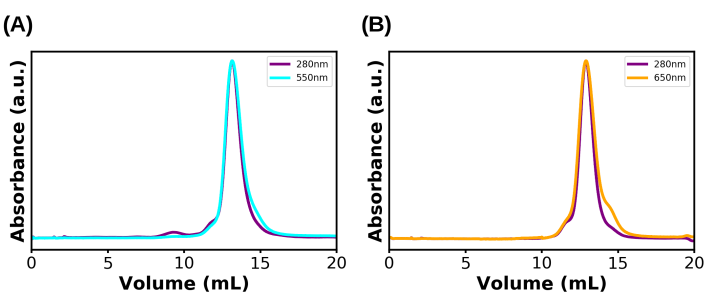
\includegraphics[width=\textwidth]{figures/chapter4/sec_cy3_cy5.pdf}
\end{center}
	\caption{\textbf{Structure of KcsA (PDB ID: 1R3J) shown from different angles}. \textbf{(A)} KcsA shown from the extracellular side of the membrane. \textbf{(B)} KcsA shown from the side. \textbf{(C)} KcsA viewed from the side with 2 monomers removed for better visualization of the selectivity filter. The oxygen atoms lining the selectivity region is rendered in Licoriche mode and the protein structures are rendered in New Cartoon mode in VMD. Each monomer of KcsA is colored in grey, blue, orange and red.}
	\label{fig:ch4_f2}
\end{figure}


Conjugation efficiency was calculated by the following equation:



\begin{equation}
	\mathrm{Conjugation\ Efficiency} = \frac{\epsilon_{dye}\alpha_{dye}}{\epsilon_{prot}\alpha_{280nm}+\epsilon_{dye}\alpha_{dye}}
\end{equation}

where $\epsilon_{prot}$ for KcsA is 33,460 cm$^{-1}$ M$^{-1}$, $\epsilon_{dye}$ = 150,000 cm$^{-1}$ M$^{-1}$ for Cy3 and 250,000 cm$^{-1}$ M$^{-1}$ Cy5, respectively, and absorbances ($\alpha_{280nm}$, $\alpha_{dye}$) were measured at 280 nm for KcsA, 550 nm for Cy3 and 650 nm for Cy5. The conjugation efficiency for both Cy3 and Cy5 samples were calculated to be ~50\%. FRET measurements were conducted with a Horiba Fluorolog-3 machine with Synapse OE-CCD Array Detector with an excitation wavelength $\lambda_{Ex}$= 500 nm. All samples contained 10 mg/mL SoyPC lipids with varying concentrations of proteins up to 10 $\mu$M.

\section{Results and Discussion}

\subsection{Kinetics of folding}

The kinetics of tetramerization of KcsA $\Delta$125 channels were examined by tracking the formation of native tetramers using an SDS resistance assay.31 The refolding protocol started with tricholoroacetic acid (TCA)-precipitated monomers solubilized with 14 mM (~0.5\% w/v) SDS at pH 6.5 (\textbf{Fig. \ref{fig:ch4_f1}A}). To initiate tetramerization, these monomers were diluted 10-fold into refolding buffer containing 14 mM asolectin liposomes. Control experiments employing dynamic light scattering verified that the liposomes remain intact after mixing with the SDS solubilized

KcsA $\Delta$125 or the 14 mM SDS buffer (Table. \ref{table:ch4_t1}). To measure refolding, aliquots of the protein-liposome mixture were removed over 25 minutes and quenched in 220 mM (~6\%) SDS buffer to arrest tetramer formation. At this high SDS concentration, liposomes were disrupted and only native tetramers persisted whereas weakly associated species were broken up and ran as monomers on SDS-PAGE gels.15-16, 31-32 The folding kinetics were quantified from the change in the gel band intensities.

\begin{table}[h]
\centering
	\caption{Folding monitored by SDS-Page gel.}
	\begin{tabular}{ccccc}
	\hline
           & WT $\Delta$125     & CC $\Delta$125      & WT FL     & CC FL                  \\
	\hline                                                                 
	\begin{tabular}[c]{@{}c@{}}Fast time\\ constant (s)\end{tabular} & \multicolumn{2}{c}{40 $\pm$ 2}     & \multicolumn{2}{c}{90 $\pm$ 10}     \\
Fast population    & \begin{tabular}[c]{@{}c@{}}0.25 $\pm$ 0.05 \\ (0.33 $\pm$ 0.05\\ 0.36 $\pm$ 0.05\\ 0.20 $\pm$ 0.05)\end{tabular} & \begin{tabular}[c]{@{}c@{}}0.86 $\pm$ 0.05\\ (0.86 $\pm$ 0.05\\ 0.83 $\pm$ 0.05\\ 0.87 $\pm$ 0.05)\end{tabular} & \begin{tabular}[c]{@{}c@{}}0.42 $\pm$ 0.04\\ (0.38 $\pm$ 0.04\\ 0.26 $\pm$ 0.04\\ 0 $\pm$ 0.04)\end{tabular} & \begin{tabular}[c]{@{}c@{}}0.55 $\pm$ 0.04\\ (0.44 $\pm$ 0.04\\ 0.16 $\pm$ 0.04\\ 0.13 $\pm$ 0.04)\end{tabular} \\
	\begin{tabular}[c]{@{}c@{}}Slow time\\ constant (s)\end{tabular} & \multicolumn{2}{c}{1500 $\pm$ 100} & \multicolumn{2}{c}{8400 $\pm$ 1600} \\
Slow population    & \begin{tabular}[c]{@{}c@{}}0.77 $\pm$ 0.03 \\ (0.70 $\pm$ 0.03\\ 0.68 $\pm$ 0.03\\ 0.83 $\pm$ 0.03)\end{tabular} & \begin{tabular}[c]{@{}c@{}}0.09 $\pm$ 0.03\\ (0.14 $\pm$ 0.03\\ 0.14 $\pm$ 0.03\\ 0.26 $\pm$ 0.03)\end{tabular} & \begin{tabular}[c]{@{}c@{}}0.59 $\pm$ 0.02\\ (0.63 $\pm$ 0.02\\ 0.76 $\pm$ 0.02\\ 1 $\pm$ 0.02)\end{tabular} & \begin{tabular}[c]{@{}c@{}}0.40 $\pm$ 0.02\\ (0.57 $\pm$ 0.02\\ 0.83 $\pm$ 0.02\\ 0.88 $\pm$ 0.02)\end{tabular} \\	\hline                
	\end{tabular}
	\label{table:ch4_t1}
	\end{table}
	
For KcsA $\Delta$125 monomers at 10 $\mu$M monomer concentration, two nearly equal refolding populations were observed, one that folded on sub-minute and another that folded on the 10 minute time scale (\textbf{Fig. \ref{fig:ch4_f3}}). Since the buildup of native tetramers is directly measured, the fast and slow appearance of native tetramers implies that there are multiple routes to the native state, rather than each phase representing a step on a sequential pathway, which would have resulted in a 10 minute lag in the buildup of tetramers.

\begin{figure}[!ht]
\begin{center}
	\includegraphics[width=\textwidth]{figures/chapter4/Fig4-2_kinetics.pdf}
\end{center}
	\caption{\textbf{Proposed KcsA folding and tetramerization.} SDS-solubilized monomers enter the liposomes and undergo rapid association into a protein-rich phase within the membrane prior to tetramerization. Oligomers can form with a native or non-native TM helical arrangement, which fold on the minute or 20 minute time scale, respectively, The rate limiting step on the faster pathway is proposed to involve the insertion of the pore helix to stabilize the tetramer in its native conformation.}
	\label{fig:ch4_f3}
\end{figure}

For the disulfide bonded CC construct, essentially all the monomers tetramerized at the fast rate (\textbf{Fig. \ref{fig:ch4_f3}}). This difference implied that the presence of unconstrained TM helices enabled the formation of a stably misfolded, slow folding species. Data for the WT and CC were fit globally, assuming the rates of the two phases were the same for the two versions. The resulting time constants were $\tau_{fast}$ = 40 $\pm$ 2 s and $\tau_{slow}$ = 1500 $\pm$ 100 s, with a 28 $\pm$ 6\% and 74 $\pm$ 6\% fast folding population for the WT and CC constructs, respectively.

\begin{figure}[!ht]
\begin{center}
	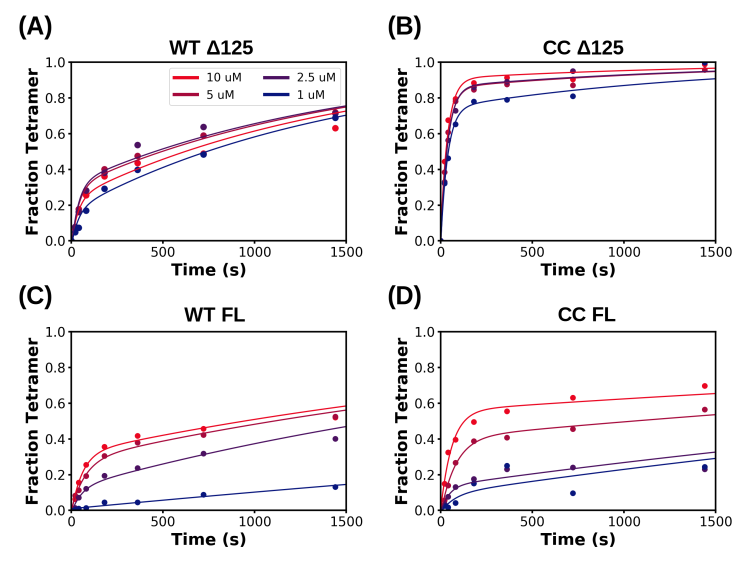
\includegraphics[width=\textwidth]{figures/chapter4/Fig4-3_conc_dependence.pdf}
\end{center}
	\caption{\textbf{Proposed KcsA folding and tetramerization.} SDS-solubilized monomers enter the liposomes and undergo rapid association into a protein-rich phase within the membrane prior to tetramerization. Oligomers can form with a native or non-native TM helical arrangement, which fold on the minute or 20 minute time scale, respectively, The rate limiting step on the faster pathway is proposed to involve the insertion of the pore helix to stabilize the tetramer in its native conformation.}
	\label{fig:ch4_f4}
\end{figure}

Next, the concentration dependence of the folding rates was studied. Interestingly, the tetramerization process, both in rate and branching ratio, appeared to be concentration independent from 1 to 10 $\mu$M within the accuracy of our measurements (\textbf{Fig. \ref{fig:ch4_f4}, Table. \ref{table:ch4_t1}}). This striking result indicates that the rate-limiting step in the folding process is a unimolecular process, despite the native state being a tetramer. If tetramerization was limited by the association of four monomers or two unstable dimers, one would have observed a 1000-fold slowing for a 10-fold decrease in concentration. As no measurable slowing was found, we propose that the oligomerization process occurs early and is fast on both routes, with the rate-limiting step representing a productive folding (fast pathway) or error-correction step (slow pathway). This proposal and the nature of this fast oligomerization process are investigated further with FRET below.

\subsection{FRET measurements suggest a formation of protein-rich phase}
The SDS folding assay indicated that the folding of both the WT and CC constructs has a minimal concentration dependence implying that the rate-limiting step is a unimolecular process. This step seems likely to occur after oligomerization in the liposomes. In principle, however, the insertion of monomers into the liposomes could be rate limiting. To test whether oligomerization is fast and occurs before the rate-limiting step, ensemble FRET measurements were carried out.

\begin{figure}[!ht]
\begin{center}
	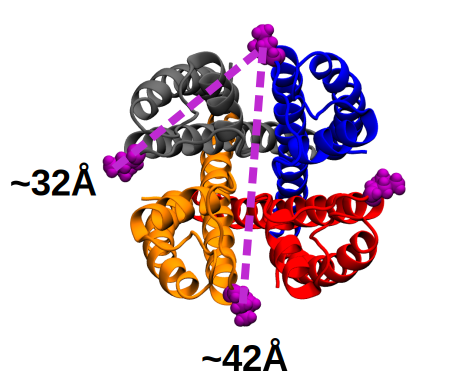
\includegraphics[width=8cm]{figures/chapter4/Fig4-4_fretpos.pdf}
\end{center}
	\caption{\textbf{Structure of KcsA with position L86C in purple.} Cy3 and Cy5 dyes were conjugated to position L86C, and mixed at a 1:1 ratio which results in two potential FRET distances of 32 and 42 Å.}
	\label{fig:ch4_f5}
\end{figure}

Dyes were first attached using thiol-labeling at a single position using a KcsA $\Delta$125 L86C variant (\textbf{Fig. \ref{fig:ch4_f5}}). Equal mixtures of donor (Cy3) and acceptor (Cy5) labeled KcsA $\Delta$125 were mixed and diluted 10-fold into the liposome mixture to initiate folding and the transfer of fluorescence was monitored (\textbf{Fig. \ref{fig:ch4_f6}}). Initially, the emission spectrum was dominated by that of the donor implying that most molecules began as isolated monomers. Upon dilution into a liposome mixture, the donor emission maximum at 570 nm was quenched by 71\% within the 10 second manual mixing dead-time while the acceptor’s emission at 680 nm increased by 7.6-fold. During the next 25 minutes over which tetramer formation occurred, only a 4\% increase in intensity was observed across the entire emission spectrum. 

\begin{figure}[!ht]
\begin{center}
	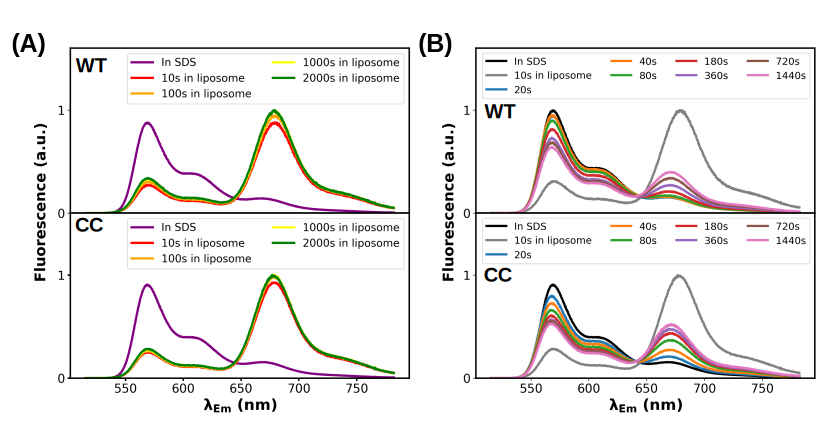
\includegraphics[width=\textwidth]{figures/chapter4/Fig4-5_fretdata.pdf}
\end{center}
	\caption{\textbf{FRET measurements of KcsA tetramerization.} \textbf{(A)} Ensemble FRET measurement of the KcsA monomer in SDS and in liposome as a function of time \textbf{(B)} Double-jump (unfold-fold-unfold) FRET measurements of KcsA refolding quenched with 10\% SDS overlaid with ‘in sds’ and ‘10s in liposome time points’ from \textbf{(A)}. Spectra are normalized to have the same value at 641 nm, an empirical iso-emissive point. Measurements are conducted at a monomer concentration of 10 $\mu$M.}
	\label{fig:ch4_f6}
\end{figure}

This biphasic FRET signal is interpreted as follows. The initial FRET increase indicates that the monomers labeled with donor and acceptor dyes rapidly associate in the liposomes prior to tetramerization. The minimal subsequent change implies that the FRET level in the rapidly associated monomers is similar to the level of folded tetramers in liposomes. The observation that most of the change in FRET signal occurred before significant tetramer formation, along with an estimate of $\sim$ 30 –- 300 monomers per liposome at 1 –- 10 $\mu$M monomer concentration, argues that most of the population forms a non-native oligomeric state upon insertion into liposomes with a FRET level comparable to that of native tetramers. The oligomers may become part of a protein-rich phase within the membrane.

To examine the possibility that FRET occurred within protein aggregates forming outside of liposomes, SDS-solubilized KcsA monomers were diluted 10-fold into water in the absence of liposomes. In this control, the overall donor fluorescence decreased 4\%, but the acceptor fluorescence spectrum only had a minimal indication of FRET (Fig. \ref), especially as compared to refolding in liposomes. The signal decrease indicates that some fraction of monomers was no longer in solution; however, more importantly, the lack of significant FRET indicates that the large observed FRET changes in the presence of liposome only came from membrane-solubilized proteins.

\begin{figure}[!ht]
\begin{center}
	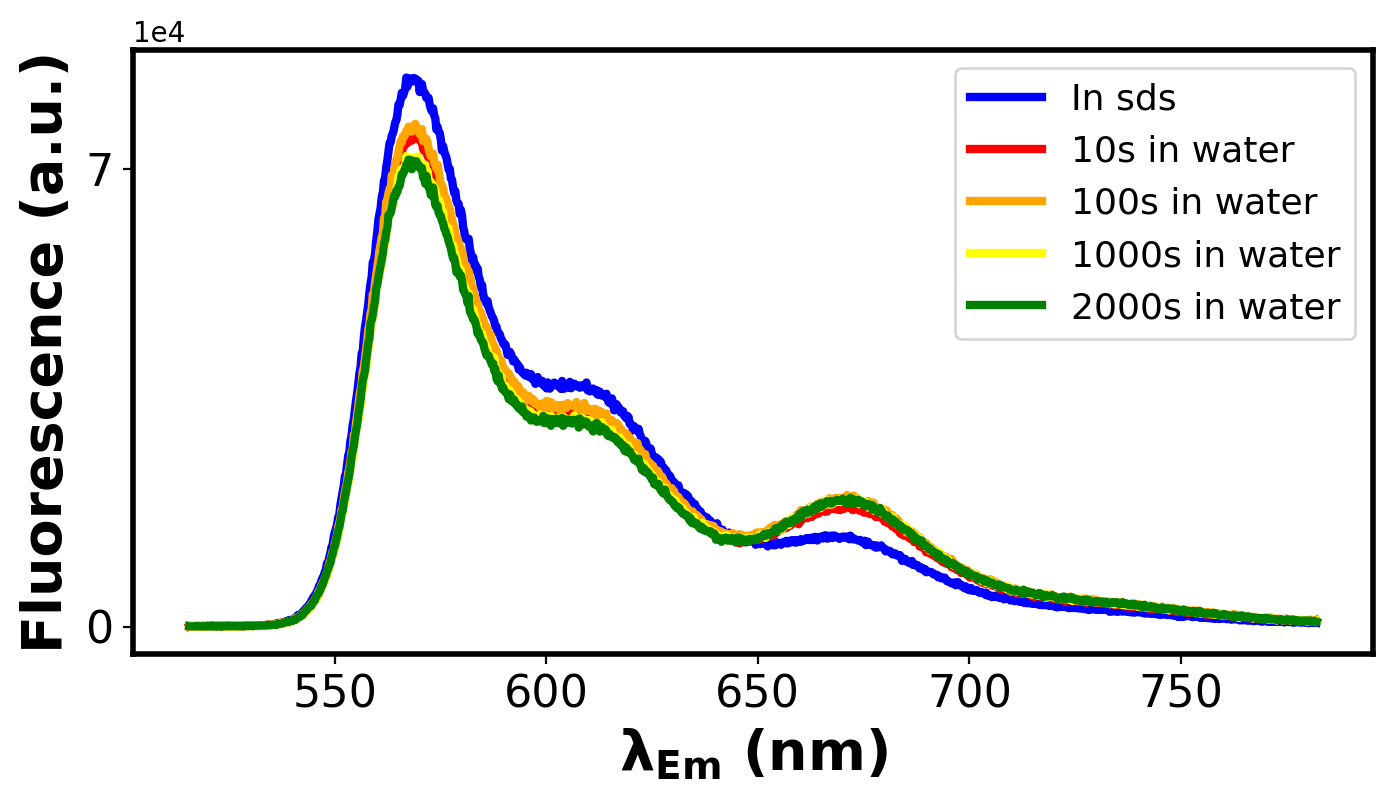
\includegraphics[width=\textwidth]{figures/chapter4/Fig4-6_watercontrol.png}
\end{center}
	\caption{\textbf{FRET measurements of KcsA tetramerization.} \textbf{(A)} Ensemble FRET measurement of the KcsA monomer in SDS and in liposome as a function of time \textbf{(B)} Double-jump (unfold-fold-unfold) FRET measurements of KcsA refolding quenched with 10\% SDS overlaid with ‘in sds’ and ‘10s in liposome time points’ from \textbf{(A)}. Spectra are normalized to have the same value at 641 nm, an empirical iso-emissive point. Measurements are conducted at a monomer concentration of 10 $\mu$M.}
	\label{fig:ch4_f7}
\end{figure}

\section{Conclusion}

Our investigation of the folding of potassium channel monomers and their role in assembly of potassium channel pores revealed a number of salient features. The MD simulations and MSM analysis indicate that for both Kv1.2 pore domain and KcsA, monomers form a heterogeneous ensemble of native and non-native states with all three helices folded and lying within the membrane. While the population of native-like states of the monomer is non-negligible (18\% for Kv1.2 and 44\% for KcsA), it is nevertheless striking that a considerable number of non-native states exists despite the substantial conformational restriction imposed by the environment; namely, the secondary structure of all three helices is retained, and the two TM helices remain inserted within the planes of the bilayer. Based on prior studies of hydrophobic matching36-39, the different lengths of TM helices presumably contribute to their tendency to separate.

This overall picture is consistent with our NMR data combined with prior thiol-labeling studies.20-21 Our attempts to generate well-resolved NMR spectra for the WT KcsA monomer inserted in nanodisc and bicelles were unsuccessful. Suspecting that the separation of the TM helices was the critical feature, a double cysteine variant was engineered to have a disulfide bond at the bottom of the two TM helices locking them into a native-like arrangement. This CC variant yielded a well-dispersed 1H-15N HSQC spectrum supporting the view that the WT’s TM helices were often separated in the monomers and formed a heterogeneous ensemble.

FRET-monitored refolding measurements of monomers passing from SDS into liposomes indicated that both WT $\Delta$125 and CC $\Delta$125 variants oligomerized well before the appearance of native tetramers. According to both SDS-resistance assays and FRET measurements, WT KcsA monomers assembled into native tetramers via two distinct kinetic paths with 40  2 and 1500  100 s. The CC variant largely if not fully lacked the slow phase. We posit that slow folding is the result of non-native packing arrangements of the TM helices that must ultimately be corrected for tetrameric assembly to proceed. The observation of slow and fast folding routes has been seen in many soluble proteins where the initial collapse step leads to species with native-like topology on a direct pathway, or to a species containing a partially misfolded structure that is slow to correct (Fig. 5).40-42

\begin{figure}[!ht]
\begin{center}
	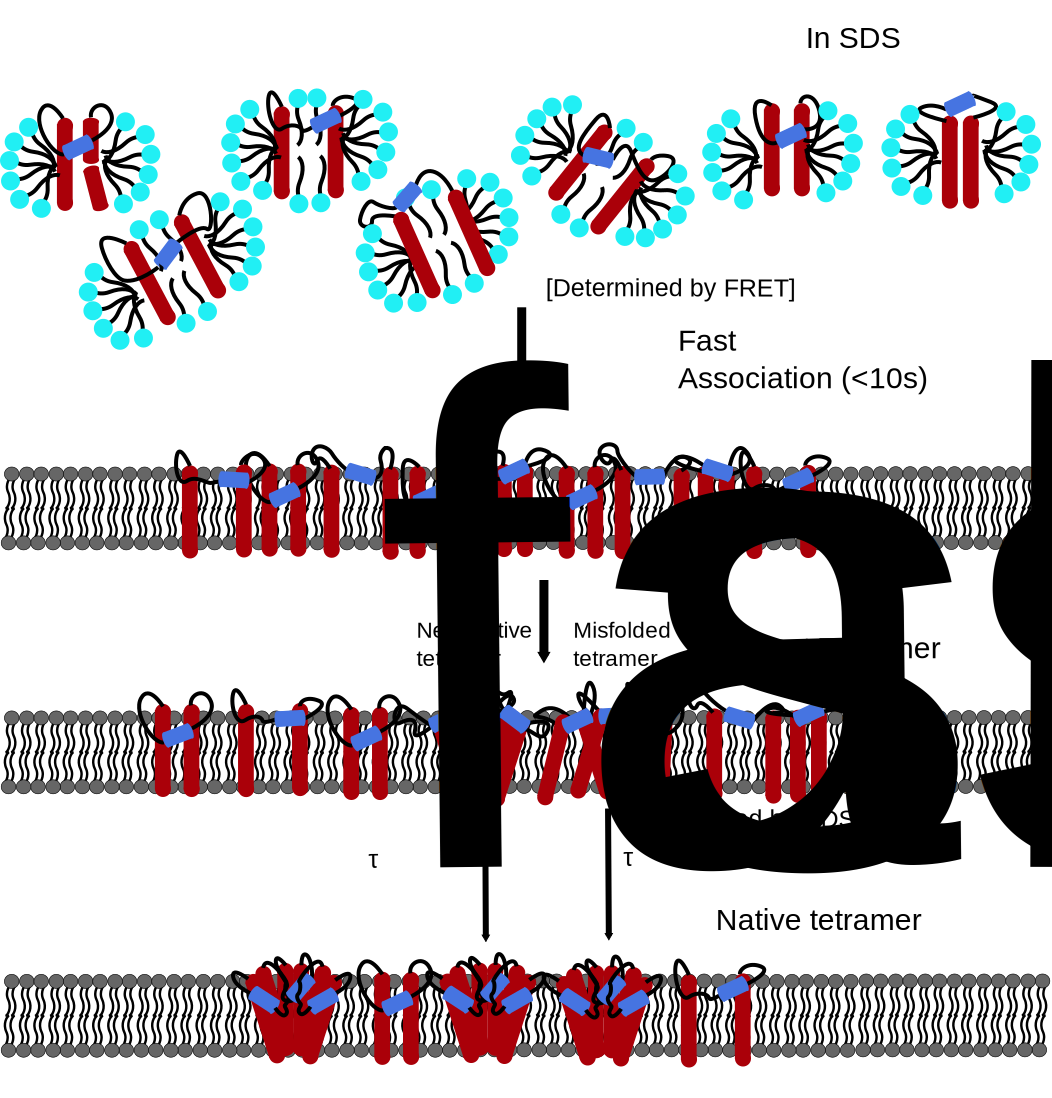
\includegraphics[width=\textwidth]{figures/chapter4/Fig4-7_summary.pdf}
\end{center}
	\caption{\textbf{Proposed KcsA folding and tetramerization.} SDS-solubilized monomers enter the liposomes and undergo rapid association into a protein-rich phase within the membrane prior to tetramerization. Oligomers can form with a native or non-native TM helical arrangement, which fold on the minute or 20 minute time scale, respectively, The rate limiting step on the faster pathway is proposed to involve the insertion of the pore helix to stabilize the tetramer in its native conformation.}
	\label{fig:ch4_f8}
\end{figure}

In spite of the channel being a tetramer, folding of the WT 125 and CC 125 constructs was concentration independent from 1 – 10 M for both the fast and slow phases, both in rate and amplitude. This observation implies that the rate-limiting step on both pathways is unimolecular. Because the FRET measurements indicated that the monomer insertion and oligomerization was relatively quick, the rate-limiting step on the fast pathway likely occurs going from an oligomer to a native tetramer. This complex transition requires the formation of the slightly twisted arrangement of the 8 TM helices, and the energetically costly opening of an aqueous channel. Final formation of native tetramers may occur in a concerted step with the association of correctly folded monomers already having the pore helices and selectivity filters positioned in a native or near-native orientation. Alternatively, this event may occur in two distinct steps, with the p-helices and selectivity filter segments folding into position only after the 8 TM have adopted their correct native arrangement. Further studies are needed to resolve this question.

The carboxy-terminal stalk domain in KcsA was tested to see if it enhanced tetramerization. In eukaryotic channels such as the Shaker voltage-activated potassium channel, the presence of the “tetramerization” T1 domain improves the rate of successful folding and assembly.13 Whereas the carboxy-terminal domain of KcsA forms a four-helix bundle that contributes to the stability of the folded tetrameric channel,43 its role in the assembly process is unclear. In other studies, the KcsA tetramerization domain alone has been shown to oligomerize in pH and concentration dependent manners44-45 as well as increase the stability of KcsA tetramers.33

However, the folding kinetics of KcsA pore domain with the tetramerization domain has not been extensively studied in the past. To our surprise, the presence of the tetramerization domain did not improve the channel’s folding behavior. For both the WT and CC variants, tetramerization became concentration dependent in a complex manner with both a reduced fast phase and lower overall yield of tetramers. One may consider that our refolding protocol with insertion into liposomes starting from an SDS-solubilized state does not properly mimic the biological context and so preclude the tetramerization domain for assisting folding. Also, the C-terminal region carries a net positive charge, which may cause a repulsion at large distance between monomers prior to tetramerization. Potentially the domain lends specificity and is more important for finding other KcsA subunits or improving the stability of tetramers once they are formed.

The folding of the potassium channels displays similar behavior to other -helical membrane proteins, having a transition state close to the native state.9-11 For example, in the force unfolding studies of GlpG pulling parallel to the bicelle surface, the transition state was closer to the native state than that observed in SDS-driven folding/unfolding studies in solution.46-47 In other SDS-based refolding studies on bacteriorhodopsin, DsbB and GlpG, the transition states were expanded.48-50 The observed difference between the force- and the SDS-driven unfolding studies may be due to the difference in the mode of denaturation as well as folding conditions (micelle or bicelle versus liposomes). Regardless, KcsA in liposomes appear to have a transition state near the native state.

The two-stage model, proposed nearly 30 years ago, has provided a useful framework for discussing membrane protein folding. The model, which posits insertion of all the TM helices followed by lateral packing, was proposed based on studies which observed that bacteriorhodopsin cut in a few pieces could still be re-assembled.51-53 With the observation of more diverse folding behaviors, a more sophisticated three-stage model10 was proposed where insertion and lateral packing of the TM helices could be followed by ligand binding, loop folding or peripheral domain insertion. This extra step is relevant to potassium channels, where the insertion of the four pore helices and the formation of the selectivity filter may be required to finalize the folding process.

For KcsA, the first two stages seem to correspond to insertion and formation of a protein-rich phase before folding into native tetrameric channels. This result brings up an interesting question in regards to membrane protein folding in general, namely, should the membrane be considered to be a good or poor solvent with respect to TM helices, defined as one where helix–lipid interactions are stronger or weaker, respectively, than helix–helix interactions. For potassium channels, a mixed behavior is observed. A protein-rich phase is detected by FRET, but the two TM helices in a monomer can dissociate from one other according to NMR (in bicelles) and MD simulations (POPC bilayers).

Potentially in the folding of other membrane proteins, non-specific or quinary interactions between TM helices also may give rise to a protein dense phase. These interactions can also occur in native structures, as seen with KcsA tetramers undergoing lateral association both in our and earlier studies.34-35 Several studies have shown that membrane proteins can alter lipid packing in the fluid liquid crystalline phase, which can in turn cause proteins to associate non-specifically in order to minimize the perturbation on the membrane.54-55 Generally, lipids may act as a marginally poor solvent for TM helices especially if the helices contain polar amino acids that are less soluble in the hydrophobic bilayer.56-62 These mixed results, along with variability of the hydrophobicity of the TM helices and the properties of the bilayer (e.g., composition, curvature, lateral pressure), suggest that solvent quality is likely system dependent. These issues have important implications to in vivo folding where helices partition between chamber of the translocon, lipid-water interface and the hydrophobic core of the membrane.63 

%% REVERT FIGURE NUMBERING %%
\renewcommand\thefigure{\thechapter.\arabic{figure}} 

%%% END CHAPTER 4 refolding studies %%%


%%% BEGIN CONCLUSION AND FUTURE DIRECTIONS %%%
\chapter{Future Directions and Conclusion}

\section{Future aims}
\subsection{Structure determination of disulfide engineered fast folding KcsA mutant}
The disulfide-bonded (CC) KcsA mutant was engineered to trap the KcsA monomers to be more native-like. Upon investigation of its kinetics, we found that this mutant folds more efficiently than the WT KcsA by avoiding misfolding of the 2 transmembrane helices. In addition, we found that the $^{1}$H-$^{15}$N-TROSY-HSQC spectrum looks much more folded than the WT spectrum. So, the question is what does the structure of this CC KcsA mutant look like in bicelles and what are its dynamics?

Through comparison of the folding kinetics of WT and CC KcsA variants we found that the misfolding of TM contributes to difference in folding kinetics between WT and CC KcsA. However, we still do not have a full understanding of how the arrangement of the pore helix affects the folding of KcsA. We hypothesize that the pore helix maintains its helicity and lay at the water-lipid interface. The pore helix maybe more dynamic than that potentially partitioning between multiple different states (solvent-exposed, lipid-water interface, and buried). With NMR peak assignments and structure, we can begin to answer some of the questions about the dynamics of the pore helix in membrane prior to tetramerization.

\subsection{Visualization of protein-rich phase}
The lipid raft hypothesis suggests that cholesterol and saturated lipids form preferential association in membranes and drive phase separation within the membrane. In return, this phase separation recruits other types of lipids and proteins for functional purposes and act as a way to compartmentalize within the membrane. In our FRET studies, we show that KcsA can non-specifically aggregate and form a protein-rich phase in the membrane.

In order to address the question of whether this protein-rich phase is real or not, we propose to use TIRF microscopy to study the formation of protein-rich phase. By looking at FRET under a microscope, we can directly observe whether protein-rich does occur in the membrane. In addition, this protein-rich phase seems to occur in soybean lipids, which we used in this thesis. It is possible that the soybean lipids act as poor solvent for KcsA causing the proteins to preferentially associate laterally in the membrane. Monitoring the formation of protein-rich phase under different lipid compositions will be informative. Perhaps, use of more anionic lipids or more unsaturated lipids can give rise to better solubilization of KcsA, which would eliminate the formation of protein-rich phase.

\subsection{Determination of the rate-limiting step in KcsA folding}
Through our concentration dependent folding kinetics studies, the rate-limiting step in KcsA folding was found to be unimolecular. This was quite surprising given the fact that KcsA is a tetramer in its native state. While we were able to show that by locking the 2 transmembrane helices in near-native state reduces KcsA's proclivity to misfold, the rate-limiting step in the reaction was not resolved. We hypothesize that the rate-limiting step correponds to the insertion of pore helices into the chamber created by 8 transmembrane helices in the membrane.

One of the ways to test our hypothesis is by introducing perturbations at the pore region to see if these perturbations affect the kinetics of the rate-limiting step. For example, potassium, barium and rubidium ions have been known to stabilize the pore structure in KcsA. In our refolding assays, none of these ions are present because they are known to strongly interact with SDS and precipitate. However, a double jump experiment could be done where SDS-solubilized KcsA monomers are first diluted into liposome solution, and then, a high concentration of potassium, barium or rubidium is injected into the refolding solution afterwards. This would give SDS-solubilized KcsA time to insert into the liposomes, so that SDS precipitation will not affect the protein. The presence of K+, Ba+ and Rb+ could increase the rate of folding by stabilizing the pore structure. In addition, we could design a disulfide bond between the pore helix and one of the 2 transmembrane helices to stabilize the native-like pore structure. This could also affect the rate-limiting step which would show that the pore region is involved in the rate-limiting step.

\section{Conclusion}
This thesis provides the first comprehensive study on potassium channel folding. The dynamics of potassium channel monomers are first studied through MD simulations and NMR spectroscopy, through which we found that the potassium channel monomers are dynamical and exists in a heterogeneous ensemble of native and non-native structures. Although the exact population level is system dependent, we found that the native state is found in 18\% and 44\% for Kv1.2 and KcsA, respectively.

In order to design a mutant that remains its near-native state when monomerized, a disulfide-bridge was engineered at the ends of the 2 transmembrane helices in KcsA. By MD simulations and NMR spectroscopy, this disulfide-bonded (CC) KcsA mutant was shown to be more native-like and homogeneous in structural states.

In our folding kinetics studies of WT and CC KcsA, we found that WT folds via 2 distinct processes, whereas the CC variant only undergoes through the faster process. This result suggests that locking the 2 transmembrane helices in native-like arrangement reduces KcsA monomers to misfold, which allows this CC variant to fold only through the faster process. This type of biphasic folding kinetics has been seen in soluble proteins as well, where the faster kinetic process represents productive folding and the slower kinetic process represents error-prone or misfolding process.

In addition, concentration dependent folding kinetics of WT and CC KcsA was studied, in which we found that both WT and CC KcsA folding is concentration independent. This is quite surprising given that the native state of KcsA is a tetramer. For a simple kinetic scheme, $ 4 [M] \rightarrow [T]$, one would expect a 1000-fold decrease in $k_{app}$ or even if dimerization was rate-limiting, one would expect 10-fold decrease when monomer concentration is changed 10-fold. This result was surprising and suggested that the rate-limiting step in folding of ptoassium channel is unimolecular.

Our concentration dependent folding kinetics study led us to hypothesize that the oligomerization process could happen very early on and folding within this near-native state is what is rate-limiting in this folding reaction. In order to investigate whether if oligomerization indeed is quick, we utilized FRET. FRET results indicated that the oligomerization process is much quicker than folding reactions indicating that KcsA might form a non-specific interaction with each other to form a dense protein-rich phase.
%% END CONCLUSION AND FUTURE DIRECTIONS %%



% Format a LaTeX bibliography
\makebibliography

% Figures and tables, if you decide to leave them to the end
%\input{figure}
%\input{table}

\end{document}


